% Options for packages loaded elsewhere
\PassOptionsToPackage{unicode}{hyperref}
\PassOptionsToPackage{hyphens}{url}
%
\documentclass[
]{article}
\usepackage{amsmath,amssymb}
\usepackage{iftex}
\ifPDFTeX
  \usepackage[T1]{fontenc}
  \usepackage[utf8]{inputenc}
  \usepackage{textcomp} % provide euro and other symbols
\else % if luatex or xetex
  \usepackage{unicode-math} % this also loads fontspec
  \defaultfontfeatures{Scale=MatchLowercase}
  \defaultfontfeatures[\rmfamily]{Ligatures=TeX,Scale=1}
\fi
\usepackage{lmodern}
\ifPDFTeX\else
  % xetex/luatex font selection
\fi
% Use upquote if available, for straight quotes in verbatim environments
\IfFileExists{upquote.sty}{\usepackage{upquote}}{}
\IfFileExists{microtype.sty}{% use microtype if available
  \usepackage[]{microtype}
  \UseMicrotypeSet[protrusion]{basicmath} % disable protrusion for tt fonts
}{}
\makeatletter
\@ifundefined{KOMAClassName}{% if non-KOMA class
  \IfFileExists{parskip.sty}{%
    \usepackage{parskip}
  }{% else
    \setlength{\parindent}{0pt}
    \setlength{\parskip}{6pt plus 2pt minus 1pt}}
}{% if KOMA class
  \KOMAoptions{parskip=half}}
\makeatother
\usepackage{xcolor}
\usepackage[margin=1in]{geometry}
\usepackage{color}
\usepackage{fancyvrb}
\newcommand{\VerbBar}{|}
\newcommand{\VERB}{\Verb[commandchars=\\\{\}]}
\DefineVerbatimEnvironment{Highlighting}{Verbatim}{commandchars=\\\{\}}
% Add ',fontsize=\small' for more characters per line
\usepackage{framed}
\definecolor{shadecolor}{RGB}{248,248,248}
\newenvironment{Shaded}{\begin{snugshade}}{\end{snugshade}}
\newcommand{\AlertTok}[1]{\textcolor[rgb]{0.94,0.16,0.16}{#1}}
\newcommand{\AnnotationTok}[1]{\textcolor[rgb]{0.56,0.35,0.01}{\textbf{\textit{#1}}}}
\newcommand{\AttributeTok}[1]{\textcolor[rgb]{0.13,0.29,0.53}{#1}}
\newcommand{\BaseNTok}[1]{\textcolor[rgb]{0.00,0.00,0.81}{#1}}
\newcommand{\BuiltInTok}[1]{#1}
\newcommand{\CharTok}[1]{\textcolor[rgb]{0.31,0.60,0.02}{#1}}
\newcommand{\CommentTok}[1]{\textcolor[rgb]{0.56,0.35,0.01}{\textit{#1}}}
\newcommand{\CommentVarTok}[1]{\textcolor[rgb]{0.56,0.35,0.01}{\textbf{\textit{#1}}}}
\newcommand{\ConstantTok}[1]{\textcolor[rgb]{0.56,0.35,0.01}{#1}}
\newcommand{\ControlFlowTok}[1]{\textcolor[rgb]{0.13,0.29,0.53}{\textbf{#1}}}
\newcommand{\DataTypeTok}[1]{\textcolor[rgb]{0.13,0.29,0.53}{#1}}
\newcommand{\DecValTok}[1]{\textcolor[rgb]{0.00,0.00,0.81}{#1}}
\newcommand{\DocumentationTok}[1]{\textcolor[rgb]{0.56,0.35,0.01}{\textbf{\textit{#1}}}}
\newcommand{\ErrorTok}[1]{\textcolor[rgb]{0.64,0.00,0.00}{\textbf{#1}}}
\newcommand{\ExtensionTok}[1]{#1}
\newcommand{\FloatTok}[1]{\textcolor[rgb]{0.00,0.00,0.81}{#1}}
\newcommand{\FunctionTok}[1]{\textcolor[rgb]{0.13,0.29,0.53}{\textbf{#1}}}
\newcommand{\ImportTok}[1]{#1}
\newcommand{\InformationTok}[1]{\textcolor[rgb]{0.56,0.35,0.01}{\textbf{\textit{#1}}}}
\newcommand{\KeywordTok}[1]{\textcolor[rgb]{0.13,0.29,0.53}{\textbf{#1}}}
\newcommand{\NormalTok}[1]{#1}
\newcommand{\OperatorTok}[1]{\textcolor[rgb]{0.81,0.36,0.00}{\textbf{#1}}}
\newcommand{\OtherTok}[1]{\textcolor[rgb]{0.56,0.35,0.01}{#1}}
\newcommand{\PreprocessorTok}[1]{\textcolor[rgb]{0.56,0.35,0.01}{\textit{#1}}}
\newcommand{\RegionMarkerTok}[1]{#1}
\newcommand{\SpecialCharTok}[1]{\textcolor[rgb]{0.81,0.36,0.00}{\textbf{#1}}}
\newcommand{\SpecialStringTok}[1]{\textcolor[rgb]{0.31,0.60,0.02}{#1}}
\newcommand{\StringTok}[1]{\textcolor[rgb]{0.31,0.60,0.02}{#1}}
\newcommand{\VariableTok}[1]{\textcolor[rgb]{0.00,0.00,0.00}{#1}}
\newcommand{\VerbatimStringTok}[1]{\textcolor[rgb]{0.31,0.60,0.02}{#1}}
\newcommand{\WarningTok}[1]{\textcolor[rgb]{0.56,0.35,0.01}{\textbf{\textit{#1}}}}
\usepackage{graphicx}
\makeatletter
\def\maxwidth{\ifdim\Gin@nat@width>\linewidth\linewidth\else\Gin@nat@width\fi}
\def\maxheight{\ifdim\Gin@nat@height>\textheight\textheight\else\Gin@nat@height\fi}
\makeatother
% Scale images if necessary, so that they will not overflow the page
% margins by default, and it is still possible to overwrite the defaults
% using explicit options in \includegraphics[width, height, ...]{}
\setkeys{Gin}{width=\maxwidth,height=\maxheight,keepaspectratio}
% Set default figure placement to htbp
\makeatletter
\def\fps@figure{htbp}
\makeatother
\setlength{\emergencystretch}{3em} % prevent overfull lines
\providecommand{\tightlist}{%
  \setlength{\itemsep}{0pt}\setlength{\parskip}{0pt}}
\setcounter{secnumdepth}{-\maxdimen} % remove section numbering
\ifLuaTeX
  \usepackage{selnolig}  % disable illegal ligatures
\fi
\usepackage{bookmark}
\IfFileExists{xurl.sty}{\usepackage{xurl}}{} % add URL line breaks if available
\urlstyle{same}
\hypersetup{
  pdftitle={Intro to multi-variable modeling},
  pdfauthor={NRES 710},
  hidelinks,
  pdfcreator={LaTeX via pandoc}}

\title{Intro to multi-variable modeling}
\author{NRES 710}
\date{Last compiled: 2024-08-19}

\begin{document}
\maketitle

\subsection{Review of class to-date!}\label{review-of-class-to-date}

We have gotten quite a bit done in class so far this semester! We are at
a good point to review what we have covered.

Many introductory statistics class for graduate students cover four
types of analysis: t-tests, ANOVA, post-hoc tests, and linear
regression. We have covered all of those topics so far as well -- but by
using the linear regression model as a vehicle to do all of those
different tests but with one cohesive framework.

I also hope that we have emphasized that the purpose of statistics is
\textbf{not} to generate \textbf{p-values} or \textbf{statistically
significant results}. Rather, the purpose of statistics is to use
\textbf{facts} to estimate \textbf{truth}. The truth we are trying to
estimate is a relationship in nature, a relationship between some
X-variable and some Y-variable.

\begin{itemize}
\tightlist
\item
  If the X-variable is continuous, we want to know what the slope is:
  how much does Y change for each unit change in X.
\item
  If the X-variable is categorical, we want to understand the difference
  between those groups. For example, consider a drug used for medical
  treatment. We want to know, for example. We don't want just know
  whether there is a statistical differenc between treatment groups. We
  want to know what the \textbf{effect} of that drug is.
\end{itemize}

One convenient feature of what we have learned so far is that all of
X-variables can be included in this general linear model:

\textbf{\(Y = \beta_0 + \beta_1 X_1 + \epsilon \sim N(0, \sigma)\)}

This model can apply to both cases, with either a continuous or
categorical X-variable.

\begin{itemize}
\tightlist
\item
  With a continuous X-variable, \(\beta_1\) is the slope.
\item
  With a categorical X-variable, \(\beta_1\) is the difference between
  the groups.

  \begin{itemize}
  \tightlist
  \item
    If you have more than two groups, you will need extra X-variables
    and betas, which can be accomplished by dummy-coding using values of
    1 and 0 to assign group ownership.
  \end{itemize}
\item
  \(\beta_0\) is always the average Y value when all other X-variables
  are 0.

  \begin{itemize}
  \tightlist
  \item
    For categorical X-variable, \(\beta_0\) is the reference group
  \item
    For a continuous X-variable, \(\beta_0\) is when X = 0.
  \end{itemize}
\end{itemize}

Assumptions of the general linear model are:

\begin{itemize}
\tightlist
\item
  Continuous Y-variable
\item
  Residuals (i.e., the error in Y) is normally distributed
\item
  If X-variable is continuous, there must be a linear relationship
  between X and Y (assumption does not apply if X-variable is
  categorical)
\item
  Homescedasticity; i.e., variance is constant along the range of
  X-values (however, t-tests and linear models can accommodate
  situations with unequal variance)
\item
  There is no autocorrelation in the Y-variable
\end{itemize}

And that's pretty much what we have covered so far.

Does anybody have any questions or is there anything you are confused
about?

\subsection{Multiple X-variables}\label{multiple-x-variables}

I have focused much of the class to date on exploring this general
linear model and how we can \textbf{extend it} to accommodate different
circumstances. And a few times I may have mentioned that one of these
extensions is to accommodate situations where we have more than one
X-variable! These might be situations where we have several categorical
X-variables of interest, or several continuous X-variables of interest,
that we think all may influence the Y-variable. You could analyze all
those X-variables separately -- and there is nothing wrong with doing
that. But, there are a lot of reasons why it would be better to analyze
all of these X-variables at the same time. And that's exactly what we
will begin to learn about today.

Let's extend the linear model to accommodate more than one X-variable:

\textbf{\(Y = \beta_0 + \beta_1 X_1 + \beta_2 X_2 + \beta_3 X_3 + ... +\epsilon \sim N(0, \sigma)\)}

\(\beta_1\) is a categorical variable with two groups, \(\beta_2\) is a
categorical variable with four groups, \(\beta_3\) is a continous
variable, and so on so forth.

In theory, you could have infinite effects! But in practice, with a
usual computer, you are restricted to having nine or ten X-variables in
the linear model.

And of course this depends on \textbf{sample size.} A good \textbf{rule
of thumb}: you will need 10 samples for every X-variable in your model.
If you have five X-variables, you should have at least 50 observations
(rows in your datafile).

A lot of people know that you can extend this model to include multiple
X-variables! But what a lot of people don't know, or struggle to
recognize, is \emph{why} you might do this\ldots{}

What are the advantages of analyzing all of your X-variables at the same
time.

\subsection{Six reasons}\label{six-reasons}

\textbf{1. It is more \emph{elegant}}.

\begin{itemize}
\tightlist
\item
  In this day and age, it is easier and more likely for you to publish a
  paper if you say: ``We ran a mixed-effects logistic regression model
  with interactions and dealt with collinearity and random
  effect\ldots{}'' Rather than to say: ``we ran a t-test''. People often
  equate complicated statistics with good science. Sometimes it does!
\item
  Othertimes, complicated statistics are not necessary. A well-designed
  experiment does not require complicated statistics!
\item
  I would say, however, that a single, multi-variable analysis is often
  much more \textbf{concise} than iterative versions of univariate
  analyses -- and I do see a lot of value in that.
\end{itemize}

\textbf{2. Swamping -- when the effect (\(\beta\)) of one variable is
masked by another}

\begin{itemize}
\tightlist
\item
  Swamping is automatically dealt with during multi-variable analyses.
\item
  A rule in statistics (axiom) -- every time you add an X into a model,
  the p-values for the X-variables already in the model should go down.
  The reason is because the p-values for your X-variables is determined
  by your error. When you add more X-variables into your model, you get
  rid of error, by explaining more noise. So, as a general rule, when
  you add more variables to a model, the p-values for other variables go
  down.
\item
  If the variable you added explains a lot, then the p-values for other
  variables should go down a lot as well!
\end{itemize}

\textbf{3. Collinearity -- when X-variables are associated with each
other}

\begin{itemize}
\tightlist
\item
  Collinearity is a big problem in ecology and natural resource
  sciences.
\item
  Collinearity is automatically dealt with in multi-variable models.
\item
  We will discuss this during the next class.
\end{itemize}

\textbf{4. Interactions -- the effect (\(\beta\)) of one X-variable
depends on the value of another X-variable}

\begin{itemize}
\tightlist
\item
  Let's say you are studying the relationship between size and age in
  two different species. You collect a bunch of data, and then you
  analyze those two different relationships in separate analyses. This
  is a valid approach.
\item
  However, what you have just done is that you have \emph{implicitly}
  assumed an interaction. You suggested that the slope of the size-age
  relationship depends upon the species.
\item
  Instead, you could have analyzed them at the same time and shown that
  those relationships are different.
\item
  Interactions are kinda\ldots{} in vogue/popular?! People think it's
  really cool/interesting to find interactions and therefore it is
  useful to examine these (?)
\item
  We will discuss these in two weeks.
\end{itemize}

\textbf{5. Blocking variables (random variables)}

\begin{itemize}
\tightlist
\item
  Similar to swamping, something that explains noise.
\item
  Sometimes we are interested in examining a core process in nature, and
  we have to measure things \textbf{in different areas}. We know that
  three different forests are different, but examining the differences
  in the forests areas is not our main purpose. We don't really care
  that the forests are different from eachother, but we want to account
  for the fact that the forests are different from eachother. We can use
  blocking or random variables to account for that random variation
  among sites, areas, forests, plots, whatever that are not relevant to
  our core process of interest.
\item
  We'll talk about this at the end of the semester.
\end{itemize}

\textbf{6. Pseudoreplication -- a process of assuming that you have more
independent samples than you really do}

\begin{itemize}
\tightlist
\item
  This is a problem in the natural sciences that many folks know about,
  but very few people understand.
\item
  A topic for the final class or two in the semester.
\end{itemize}

\subsection{How multi-variable models
work}\label{how-multi-variable-models-work}

\textbf{\(Y = \beta_0 + \beta_1 X_1 + \beta_2 X_2 + \epsilon \sim N(0, \sigma)\)}

\textbf{Y = Size}\\
\textbf{\(X_1\) = Age} (continuous)\\
\textbf{\(X_2\) = Sex} (categorical)

This model has traditionally been called `\textbf{Analysis of Covariance
(ANCOVA)}'.

If you have more than one categorical X, that model has historically
been called a `\textbf{Multi-factor ANOVA}'.

I don't expect you to know these terms, because I won't use them. But
you might hear them or see them, so giving them here for context\ldots{}

If you have more than one continuous X, that model has historically been
called a `\textbf{Multiple Regression}' -- as opposed to our simple
linear regression with one X-variable.

However, we can call them all \textbf{`General Linear Models'} -- much
easier!

\textbf{\(Y = \beta_0 + \beta_1 Age + \beta_2 Sex + \epsilon \sim N(0, \sigma)\)}

\textbf{Y = Size}\\
\textbf{\(X_1\) = Age} (continuous)\\
\textbf{\(X_2\) = Sex} (categorical; male = 1)

Important point: when we run this model, it does not change the meanings
of the betas at all! They are still interpretted the same ways as we
have interpretted them before.

\begin{itemize}
\tightlist
\item
  The meaning of \(\beta_1\) is the effect (slope) of age on size -- or
  the slope of the age-size relationship
\item
  The meaning of \(\beta_2\) is the difference between male and females
  (or, the effect of being male compared to the reference, female).
\end{itemize}

The fact that we have an age effect in the model does not change our
interpretation of the sex effect -- or vice versa!

So, this `more complicated model' does not make it harder to interpet
these betas -- they still have the same meaning!

Let's see what this looks like.

\subsection{Conceptual example}\label{conceptual-example}

Continuing the size (Y) by age (X) and sex (X) example, consider this
plot of data:

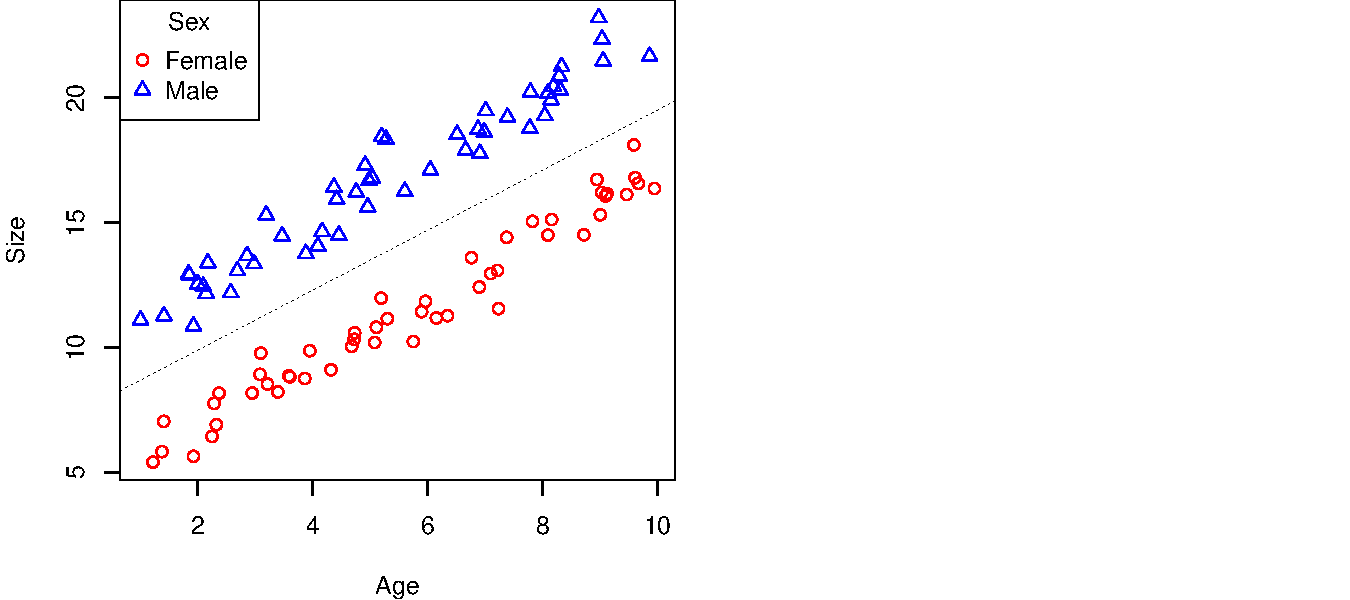
\includegraphics{lecture_12_files/figure-latex/example1-1.pdf}

One of the things I want to point out is that\ldots{} we can run a
simple regression between age and size!

\textbf{Q:} If I did that, where would the line be? \textbf{Right down
the middle -- between the two clusters of data.}

\textbf{Q:} Would we get a good estimate of the age-sex relationship?
\textbf{Yes!} It would be pretty good.

\textbf{Error:} But, our \textbf{error} would be pretty large**. We can
indicate this with a normal curve overlayed on top of the regression
line and the spread of the data.

Now let's consider what would happen if we run the multivariable model.
What's actually going to happen is we are going to get \textbf{two
lines!} One for females, and one for males. Let's break up the model and
examine this:

\textbf{\(Y(female) = \beta_0 + \beta_1 Age + \cancel{\beta_2 * 0} + \epsilon \sim N(0, \sigma)\)}

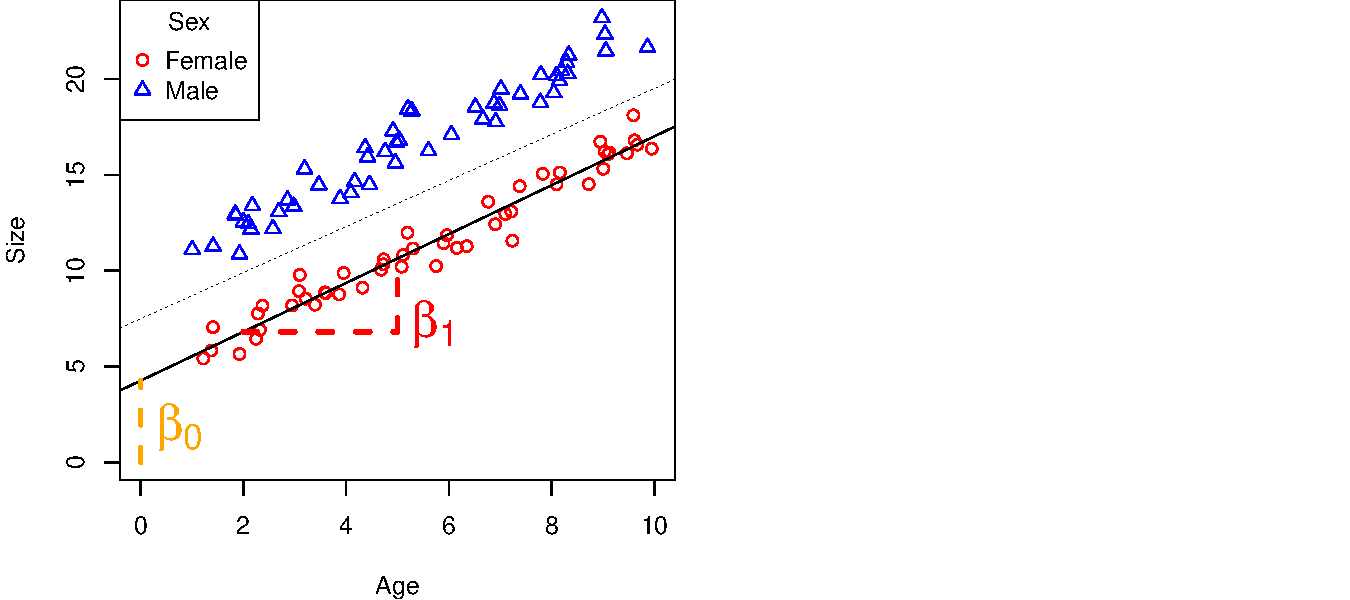
\includegraphics{lecture_12_files/figure-latex/example2-1.pdf}

What happens to the Beta2 * Sex term for females? It goes away, because
Sex = 0 for females. So now we have a line just for female data!

\textbf{Error:} Our \textbf{error} for this line will be \textbf{much
smaller} than for a line for all the data. We can indicate this with
smaller normal curves overlayed on top of the data and regression line
for females.

The Y-intercept for this line is Beta0, the slope for this line is
Beta1.

Now let's examine this for males.

\textbf{\(Y(male) = \beta_0 + \beta_1 Age + \beta_2 * 1 + \epsilon \sim N(0, \sigma)\)}

Let's rearrange the equation to move \(\beta_2\) over next to
\(\beta_0\). We can do that because these are both just being added.

\textbf{\(Y(male) = (\beta_0 + \beta_2) + \beta_1 Age + \epsilon \sim N(0, \sigma)\)}

So basically what this is saying is that our intercept is now
\(\beta_0 + \beta_2\). In other words, the intercept for the male
equation is the female intercept (\(\beta_0\)) plus the difference of
being male (\(\beta_2\)).

The slope for the male line is the same term as the slope for the female
line (\$\beta\_1)!

We can also visualize this on our graph:

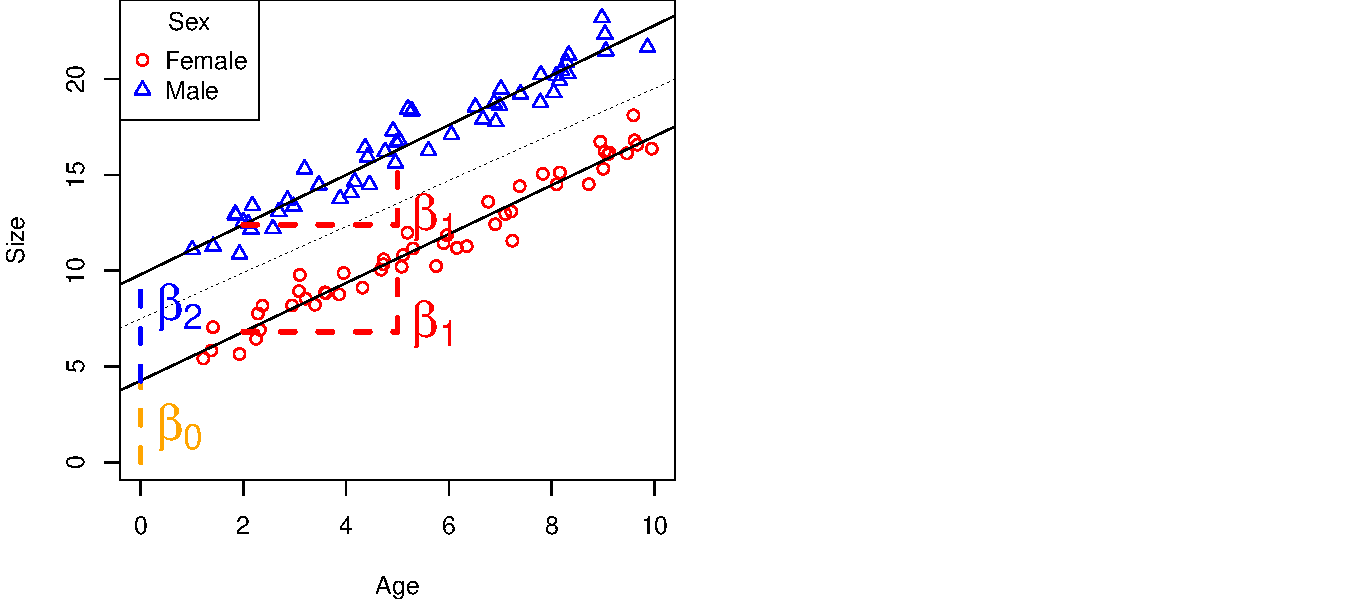
\includegraphics{lecture_12_files/figure-latex/example3-1.pdf}

\textbf{Error:} As with the line for females, our \textbf{error} for
this line will be \textbf{much smaller} than for a line for all the
data. We can indicate this with smaller normal curves overlayed on top
of the data and regression line for females.

Ultimately, by using this equation, we can capture all of the meaningful
variation in the data, and it does so by allowing for much smaller error
than more simple models.

The meaning of the betas has not changed. \(\beta_1\) is the slope for
both lines, and \(\beta_2\) is the difference between the groups. Notice
that \(\beta_2\) is not just the difference between the groups at age of
zero, it's the difference everywhere! It's constant along the variation
of the continuous X-variable.

\textbf{Questions?}

Previously I mentioned one of the reasons we like multi-variable
analysis is it automatically accounts for \textbf{swamping}. For
example, if we run univariate analysis (a model with one X-variable), we
may not observe a statistically significant result because a ton of
variation in the system is explained by another X-variable. The result
is `swamped' out by the other X-variable that we did not include.
\textbf{The effect of one X-variable is masked by another}.

By adding in multiple X-variables, multi-variable analysis automatically
deals with swamping.

Because we have decreased the error related to all of the terms in our
model, we have also decreased the p-values for each term.

It's also entirely possible that if we had not included one of the
X-variables in our model, we might NOT have recovered good estimates of
the \(\beta\) and instead failed to reject the null hypothesis of no
effect.

For example, looking back at our original line fit to all of the data.
We may have recovered a significant slope for this line, but our would
have been higher, our confidence intervals would have been larger, and
our estimate would not have been certain.

What if we wouldn't have included age in the model?

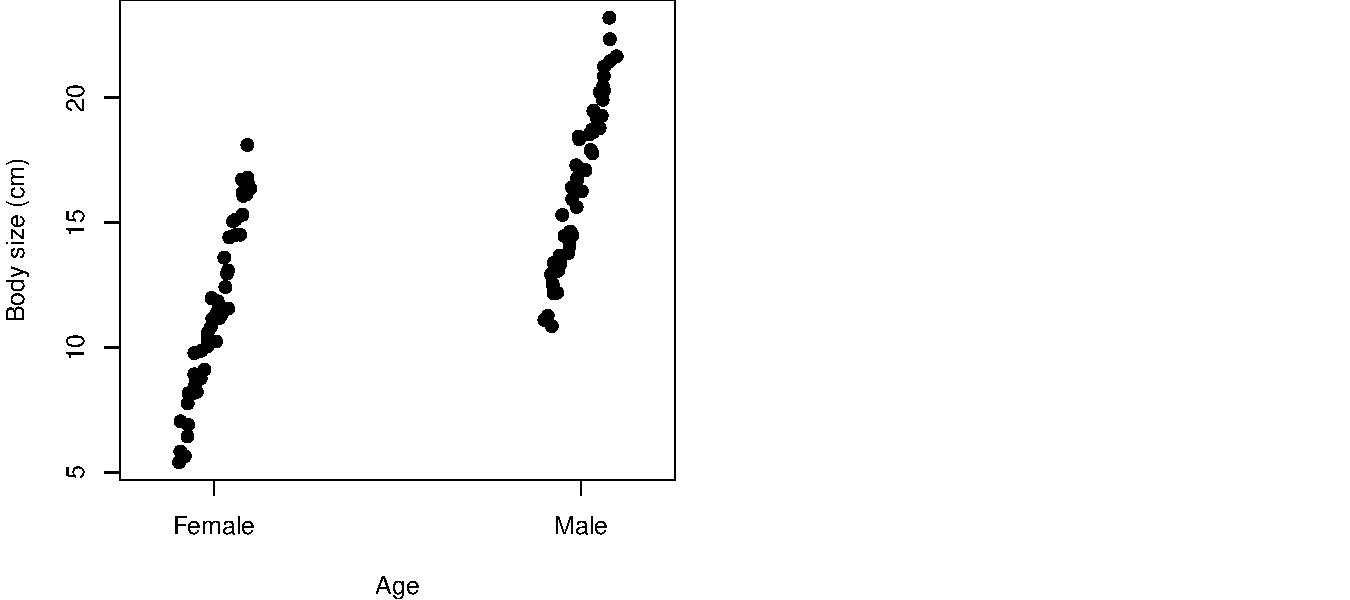
\includegraphics{lecture_12_files/figure-latex/example4-1.pdf}

\textbf{Q:} Are these groups going to be significantly different from
eachother?

Maybe\ldots{} but there is a lot of noise here, and the groups overlap
eachother. A linear model of sex alone {[}e.g., lm(Size
\textasciitilde{} Sex){]} may not return significance and thus we would
fail to reject the null hypothesis of no difference between groups.

\textbf{Takehome message:} by accounting for how both age and sex
influences size in the model, our models will, in general, explain more
variation and better recovery real, statistically-significant results.
This helps minimize negative effects of swamping.

\subsection{Multi-variable models in
R}\label{multi-variable-models-in-r}

\subsubsection{Simple analysis}\label{simple-analysis}

So let's load up some data in R and take a look at it.

\begin{Shaded}
\begin{Highlighting}[]
\CommentTok{\# Load in the data and take a look at it}
\NormalTok{datum }\OtherTok{\textless{}{-}} \FunctionTok{read.csv}\NormalTok{(}\StringTok{"lecture\_12\_dataset1.csv"}\NormalTok{)}

\CommentTok{\# Take a look at it}
\FunctionTok{head}\NormalTok{(datum)}
\FunctionTok{tail}\NormalTok{(datum)}
\end{Highlighting}
\end{Shaded}

The data include:

\begin{itemize}
\tightlist
\item
  observations of animals of different ages (1-10 years old, roughly)
\item
  different sexes (males and females)
\item
  a dummy-coded variable for sex (0 = female, 1 = male)
\item
  body size
\end{itemize}

What was the \textbf{Truth} used to simulate these data? The code to
simulate these data are included at the bottom of this page. But, here's
a quick summary:

\textbf{Truth:}

\begin{itemize}
\tightlist
\item
  \(\beta_1\) = 1.5 (age effect)
\item
  \(\beta_2\) = 2.5 (beta for sex; a.k.a., the effect of being male)
\item
  \(\beta_0\) = 4 (y-intercept for reference group)
\item
  \(\sigma\) = 0.8
\end{itemize}

Let's plot it! Start with the effect of sex on size.

\begin{Shaded}
\begin{Highlighting}[]
\CommentTok{\# Plot the effect of sex on size}
\FunctionTok{plot}\NormalTok{(Size }\SpecialCharTok{\textasciitilde{}} \FunctionTok{as.factor}\NormalTok{(Sex), }\AttributeTok{data =}\NormalTok{ datum)}
\end{Highlighting}
\end{Shaded}

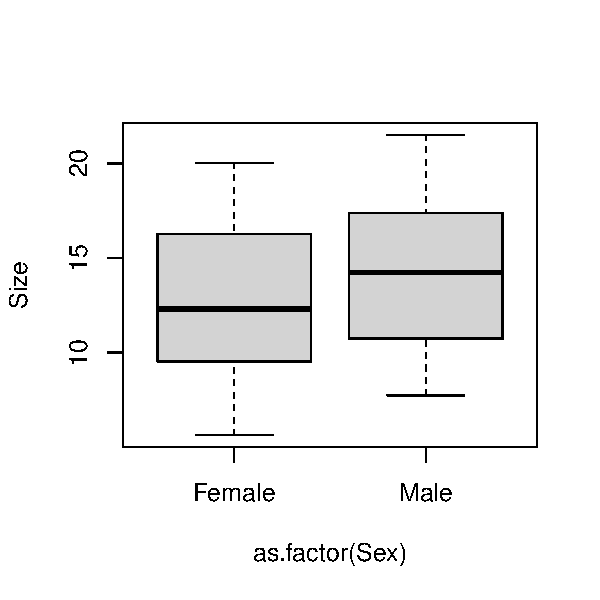
\includegraphics{lecture_12_files/figure-latex/analysis_2-1.pdf}

Yeesh! A lot of noise here, a lot of interlap between our two groups.
This is not particularly useful.

Let's look at the effect of age on size.

\begin{Shaded}
\begin{Highlighting}[]
\CommentTok{\# Plot the effect of sex on size}
\FunctionTok{plot}\NormalTok{(Size }\SpecialCharTok{\textasciitilde{}}\NormalTok{ Age, }\AttributeTok{data =}\NormalTok{ datum)}
\end{Highlighting}
\end{Shaded}

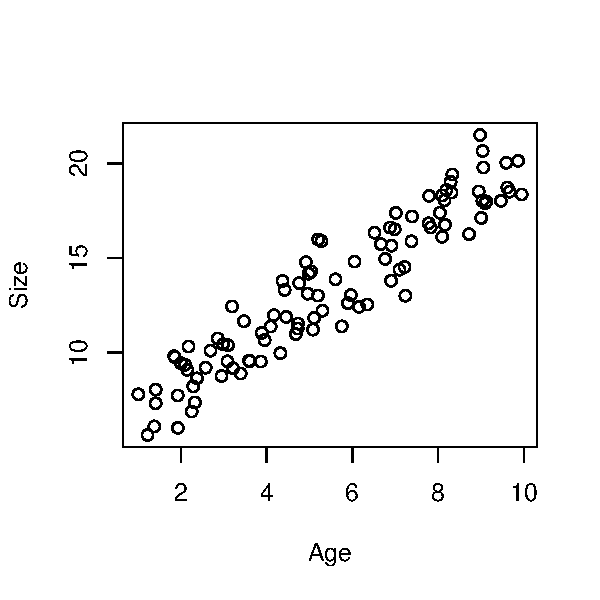
\includegraphics{lecture_12_files/figure-latex/analysis_3-1.pdf}

Can we see a difference between males and females? Not really. Maybe we
could if we plotted the points using different colors or point types for
each sex. But there is not a clear separation of points suggestion of
two groups looking at it like this.

Let's now start by running a regression between \textbf{sex} and
\textbf{size}.

\begin{Shaded}
\begin{Highlighting}[]
\CommentTok{\# Simple regression between size and sex }
\NormalTok{results1 }\OtherTok{\textless{}{-}} \FunctionTok{lm}\NormalTok{(Size }\SpecialCharTok{\textasciitilde{}}\NormalTok{ Sex, }\AttributeTok{data =}\NormalTok{ datum)}
\FunctionTok{summary}\NormalTok{(results1)}
\end{Highlighting}
\end{Shaded}

\begin{verbatim}
## 
## Call:
## lm(formula = Size ~ Sex, data = datum)
## 
## Residuals:
##    Min     1Q Median     3Q    Max 
## -6.982 -3.126 -0.158  3.306  7.388 
## 
## Coefficients:
##             Estimate Std. Error t value Pr(>|t|)    
## (Intercept)   12.638      0.551   22.93   <2e-16 ***
## SexMale        1.598      0.779    2.05    0.043 *  
## ---
## Signif. codes:  0 '***' 0.001 '**' 0.01 '*' 0.05 '.' 0.1 ' ' 1
## 
## Residual standard error: 3.9 on 98 degrees of freedom
## Multiple R-squared:  0.0411, Adjusted R-squared:  0.0314 
## F-statistic: 4.21 on 1 and 98 DF,  p-value: 0.043
\end{verbatim}

Remember, truth for the effect of being male, \(\beta_2\), was 2.5. Our
results here suggest that this effect is 1.5. But it is statistically
significant -- although barely (p = 0.04). Our confidence limits are
about \textasciitilde1.5 (2 * SE). So our best guess from this model is
that males are about 1.5 kg larger than females (+/- 1.5). This is a
pretty noisy estimate -- but it does contain truth, which was 2.5.

Notice the residual standard error is about \textasciitilde4. Truth was
1! So this is about four times larger than truth. There is a lot of
extra noise (error) in this simple model! Noise is often not just random
variation, but there might be other information that might explains that
noise in size. In this case, a lot of the variation in size is driven by
age, while very little information is driven by sex.

\textbf{Q:} How much variation in size is explained by sex? \textbf{Only
4\%!} The multiple \(R^2\).

Let's now start by running a regression between \textbf{age} and
\textbf{size}.

\begin{Shaded}
\begin{Highlighting}[]
\CommentTok{\# Plot}
\FunctionTok{plot}\NormalTok{(Size }\SpecialCharTok{\textasciitilde{}}\NormalTok{ Age, }\AttributeTok{data =}\NormalTok{ datum)}
\end{Highlighting}
\end{Shaded}

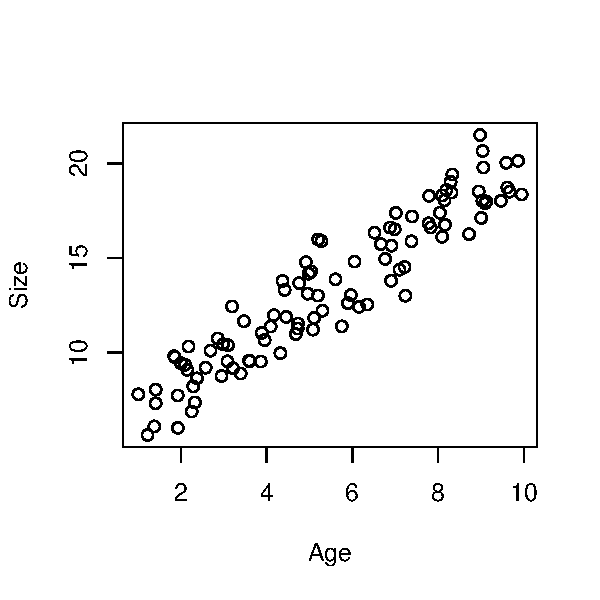
\includegraphics{lecture_12_files/figure-latex/analysis_5-1.pdf}

\begin{Shaded}
\begin{Highlighting}[]
\CommentTok{\# Simple regression between size and age }
\NormalTok{results2 }\OtherTok{\textless{}{-}} \FunctionTok{lm}\NormalTok{(Size }\SpecialCharTok{\textasciitilde{}}\NormalTok{ Age, }\AttributeTok{data =}\NormalTok{ datum)}
\FunctionTok{summary}\NormalTok{(results2)}
\end{Highlighting}
\end{Shaded}

\begin{verbatim}
## 
## Call:
## lm(formula = Size ~ Age, data = datum)
## 
## Residuals:
##    Min     1Q Median     3Q    Max 
## -2.975 -1.087 -0.011  1.074  2.978 
## 
## Coefficients:
##             Estimate Std. Error t value Pr(>|t|)    
## (Intercept)   5.4549     0.3158    17.3   <2e-16 ***
## Age           1.4548     0.0522    27.9   <2e-16 ***
## ---
## Signif. codes:  0 '***' 0.001 '**' 0.01 '*' 0.05 '.' 0.1 ' ' 1
## 
## Residual standard error: 1.33 on 98 degrees of freedom
## Multiple R-squared:  0.888,  Adjusted R-squared:  0.887 
## F-statistic:  777 on 1 and 98 DF,  p-value: <2e-16
\end{verbatim}

The effect of Age is 1.45 (+/- 0.10), which is \textbf{great} because it
is very close to and overlaps with truth (1.5)! This is also highly
significant, P = 2x10\^{}-16.

We don't really need to include sex in the model to get a good estimate
of the effect of age. Why\ldots?

Because age explains 88\% of the variation in size! We get pretty good
estimates of this effect of age on size without including information on
sex. However, if we do, this R\^{}2 value will increase also!

Let's run the full model.

\begin{Shaded}
\begin{Highlighting}[]
\CommentTok{\# Simple regression between size and age }
\NormalTok{results3 }\OtherTok{\textless{}{-}} \FunctionTok{lm}\NormalTok{(Size }\SpecialCharTok{\textasciitilde{}}\NormalTok{ Age }\SpecialCharTok{+}\NormalTok{ Male, }\AttributeTok{data =}\NormalTok{ datum)}
\FunctionTok{summary}\NormalTok{(results3)}
\end{Highlighting}
\end{Shaded}

\begin{verbatim}
## 
## Call:
## lm(formula = Size ~ Age + Male, data = datum)
## 
## Residuals:
##     Min      1Q  Median      3Q     Max 
## -1.9445 -0.4822 -0.0336  0.4328  1.8820 
## 
## Coefficients:
##             Estimate Std. Error t value Pr(>|t|)    
## (Intercept)   4.1900     0.2013    20.8   <2e-16 ***
## Age           1.4872     0.0299    49.7   <2e-16 ***
## Male          2.1748     0.1528    14.2   <2e-16 ***
## ---
## Signif. codes:  0 '***' 0.001 '**' 0.01 '*' 0.05 '.' 0.1 ' ' 1
## 
## Residual standard error: 0.762 on 97 degrees of freedom
## Multiple R-squared:  0.964,  Adjusted R-squared:  0.963 
## F-statistic: 1.29e+03 on 2 and 97 DF,  p-value: <2e-16
\end{verbatim}

\textbf{Q:} What are we seeing that is different about this output than
the previous two outputs?

\begin{itemize}
\tightlist
\item
  The effect of age is much closer to truth! And still highly
  significant.
\item
  The effect of male is now much closer to truth!

  \begin{itemize}
  \tightlist
  \item
    The simple sex model had a p-value = 0.04, but now it's 2e-16! We
    drastically increased our ability to estimate this significant
    effect.
  \end{itemize}
\item
  The y-intercept for the reference group (females) is closer to truth
  (4.18 vs.~4).
\item
  \(R^2\) value jumped up to 0.96! We are now explaining more
  information in size than either of the previous two simple models
  (0.04, 0.88) combined. This model, as a whole, explains 96\% of the
  variation in size.
\item
  Standard error estimate is much closer! 0.76 is closer to truth
  (0.80).
\end{itemize}

This is a good illustration of \textbf{swamping}. Swamping occurs when
the effect of one variable is drowned out by another variables effect.
Univariate analysis may fail to recover all of the significant effects;
our ability to measure statistically significant effects can be swamped
out by other variables. By including all of these variables in a single
model, we can correctly account for variation explained by different
variables and appropriately measure and identify these
statistically-significant effects.

This is an advantage of using multi-variable analysis: by analyze all of
the variables together, it improves our ability to estimate truth!

NOTE: something weird is happening. Even now with this improved model,
our effect of age (2.17; +/- 0.3, 95\% CI) does not overlap with truth!!

Sometimes this happens due to random chance during data simulation!
Basically, the simulation process ended up simulating pretty extreme
data for the male effect in this case, due to random chance. Given our
sample size and effect size, our estimate does not overlap in truth,
even after correctly specifying the true model. This happens maybe 1 out
of every 20 simulations. That's just part of the randomness of data and
science!

\textbf{Reporting results}

One sentence for every X-variable, and those sentences will be the same
as we have used before.

For the continuous X-variable, provide a results sentence for a
continuous variable. ``For each 1 year in increase in age, we observed a
1.49 (+/-0.06; +/-95\% CI) kg increase in body size (P \textless{}
2e-16).''

For the categorical X-variable, provide a results sentence for that
variable illustrating the difference between sexes. ``We also found that
body size of males was 2.17 (+/-0.30; +/-95\% CI) kg heavier than
females (P \textless{} 2e-16).''

One sentence for each variable, and the same sentences we already know!

\subsubsection{More complex analysis}\label{more-complex-analysis}

Let's assume the same dataset as before, but we now have a third group:
hermaphrodites. Individual animals with sexual reproductive organs for
both sexes.

\begin{Shaded}
\begin{Highlighting}[]
\CommentTok{\# Load in the data and take a look at it}
\NormalTok{datum }\OtherTok{\textless{}{-}} \FunctionTok{read.csv}\NormalTok{(}\StringTok{"lecture\_12\_dataset2.csv"}\NormalTok{)}

\CommentTok{\# Take a look at it}
\FunctionTok{head}\NormalTok{(datum)}
\FunctionTok{tail}\NormalTok{(datum)}

\CommentTok{\# Make sure Sex is a factor}
\NormalTok{datum}\SpecialCharTok{$}\NormalTok{Sex }\OtherTok{\textless{}{-}} \FunctionTok{as.factor}\NormalTok{(datum}\SpecialCharTok{$}\NormalTok{Sex)}
\end{Highlighting}
\end{Shaded}

I simulated these data using the same `truth' as before for males and
females; males were 2.5 kg larger than females on average. But now I
simulated the third hermaphrodite group where hermaphrodites are 5 kg
larger than females on average.

\begin{Shaded}
\begin{Highlighting}[]
\CommentTok{\# Plot the data}
\FunctionTok{plot}\NormalTok{(Size }\SpecialCharTok{\textasciitilde{}} \FunctionTok{as.factor}\NormalTok{(Sex), }\AttributeTok{data =}\NormalTok{ datum)}
\end{Highlighting}
\end{Shaded}

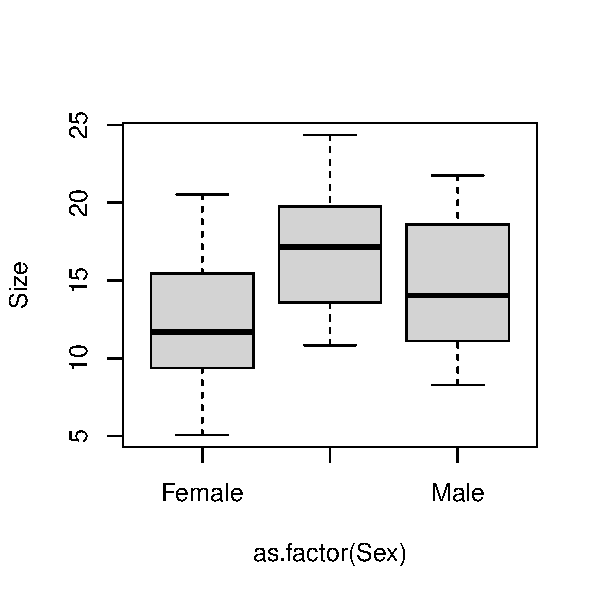
\includegraphics{lecture_12_files/figure-latex/analysis_2_2-1.pdf}

\begin{Shaded}
\begin{Highlighting}[]
\CommentTok{\# Plot again}
\FunctionTok{plot}\NormalTok{(Size }\SpecialCharTok{\textasciitilde{}}\NormalTok{ Age, }\AttributeTok{data =}\NormalTok{ datum)}
\end{Highlighting}
\end{Shaded}

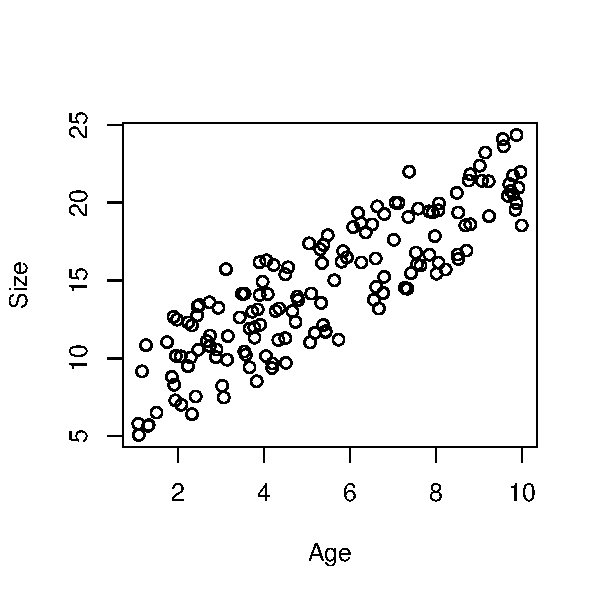
\includegraphics{lecture_12_files/figure-latex/analysis_2_2-2.pdf}

Let's jump straight to the full model:

\begin{Shaded}
\begin{Highlighting}[]
\CommentTok{\# Multi{-}variable analysis}
\NormalTok{results }\OtherTok{\textless{}{-}} \FunctionTok{lm}\NormalTok{(Size }\SpecialCharTok{\textasciitilde{}}\NormalTok{ Age }\SpecialCharTok{+}\NormalTok{ Sex, }\AttributeTok{data =}\NormalTok{ datum)}
\FunctionTok{summary}\NormalTok{(results)}
\end{Highlighting}
\end{Shaded}

\begin{verbatim}
## 
## Call:
## lm(formula = Size ~ Age + Sex, data = datum)
## 
## Residuals:
##     Min      1Q  Median      3Q     Max 
## -2.0316 -0.5018 -0.0379  0.5908  2.0127 
## 
## Coefficients:
##                  Estimate Std. Error t value Pr(>|t|)    
## (Intercept)        4.0078     0.1811    22.1   <2e-16 ***
## Age                1.5021     0.0257    58.4   <2e-16 ***
## SexHermaphrodite   5.0301     0.1629    30.9   <2e-16 ***
## SexMale            2.6028     0.1629    16.0   <2e-16 ***
## ---
## Signif. codes:  0 '***' 0.001 '**' 0.01 '*' 0.05 '.' 0.1 ' ' 1
## 
## Residual standard error: 0.815 on 146 degrees of freedom
## Multiple R-squared:  0.968,  Adjusted R-squared:  0.967 
## F-statistic: 1.45e+03 on 3 and 146 DF,  p-value: <2e-16
\end{verbatim}

So our interpretation of this is essentially the same as our
interpretation before.

\begin{itemize}
\tightlist
\item
  We have a continuous effect of age, which is different due to random
  variables but still a good estimate.
\end{itemize}

\textbf{Q:} What is the interpretation for the `SexHerma' effect?
\textbf{Difference between hermaphrodites and females}. We would use our
standard sentence to explain that.

\textbf{Q:} What is the interpretation for the `SexMale' effect?
\textbf{Difference between males and females}. Again, standard sentence
to explain that.

\textbf{Q:} What if we want to know the difference between males and
hermaphrodites? \textbf{Change the reference}

Let's do that real quick.

\begin{Shaded}
\begin{Highlighting}[]
\CommentTok{\# Use the relevel function to change order of sex}
\NormalTok{results2 }\OtherTok{\textless{}{-}} \FunctionTok{lm}\NormalTok{(Size }\SpecialCharTok{\textasciitilde{}}\NormalTok{ Age }\SpecialCharTok{+} \FunctionTok{relevel}\NormalTok{(Sex, }\AttributeTok{ref =} \StringTok{"Male"}\NormalTok{), }\AttributeTok{data =}\NormalTok{ datum)}
\FunctionTok{summary}\NormalTok{(results2)}
\end{Highlighting}
\end{Shaded}

\begin{verbatim}
## 
## Call:
## lm(formula = Size ~ Age + relevel(Sex, ref = "Male"), data = datum)
## 
## Residuals:
##     Min      1Q  Median      3Q     Max 
## -2.0316 -0.5018 -0.0379  0.5908  2.0127 
## 
## Coefficients:
##                                         Estimate Std. Error t value Pr(>|t|)    
## (Intercept)                               6.6106     0.1810    36.5   <2e-16 ***
## Age                                       1.5021     0.0257    58.4   <2e-16 ***
## relevel(Sex, ref = "Male")Female         -2.6028     0.1629   -16.0   <2e-16 ***
## relevel(Sex, ref = "Male")Hermaphrodite   2.4273     0.1629    14.9   <2e-16 ***
## ---
## Signif. codes:  0 '***' 0.001 '**' 0.01 '*' 0.05 '.' 0.1 ' ' 1
## 
## Residual standard error: 0.815 on 146 degrees of freedom
## Multiple R-squared:  0.968,  Adjusted R-squared:  0.967 
## F-statistic: 1.45e+03 on 3 and 146 DF,  p-value: <2e-16
\end{verbatim}

I haven't changed anything about age, but just replaced sex with the
relevel function inside our linear model.

And voila! Here is our difference between hermaphrodites and males.

\begin{Shaded}
\begin{Highlighting}[]
\CommentTok{\# Back to original results}
\FunctionTok{summary}\NormalTok{(results)}
\end{Highlighting}
\end{Shaded}

\begin{verbatim}
## 
## Call:
## lm(formula = Size ~ Age + Sex, data = datum)
## 
## Residuals:
##     Min      1Q  Median      3Q     Max 
## -2.0316 -0.5018 -0.0379  0.5908  2.0127 
## 
## Coefficients:
##                  Estimate Std. Error t value Pr(>|t|)    
## (Intercept)        4.0078     0.1811    22.1   <2e-16 ***
## Age                1.5021     0.0257    58.4   <2e-16 ***
## SexHermaphrodite   5.0301     0.1629    30.9   <2e-16 ***
## SexMale            2.6028     0.1629    16.0   <2e-16 ***
## ---
## Signif. codes:  0 '***' 0.001 '**' 0.01 '*' 0.05 '.' 0.1 ' ' 1
## 
## Residual standard error: 0.815 on 146 degrees of freedom
## Multiple R-squared:  0.968,  Adjusted R-squared:  0.967 
## F-statistic: 1.45e+03 on 3 and 146 DF,  p-value: <2e-16
\end{verbatim}

What if I asked you to give a p-value for the significance of the sex
variable as a whole? Before, we used the p-value in the bottom-right
hand output of our results. But now this new modeling approach also has
a continuous X-variable involved, so this p-value now relates to the
significance of our larger multi-variable modeling approach, which
includes both age and sex.

You could do it this way:

\begin{Shaded}
\begin{Highlighting}[]
\CommentTok{\# ANOVA}
\FunctionTok{anova}\NormalTok{(results)}
\end{Highlighting}
\end{Shaded}

\begin{verbatim}
## Analysis of Variance Table
## 
## Response: Size
##            Df Sum Sq Mean Sq F value Pr(>F)    
## Age         1   2254    2254    3398 <2e-16 ***
## Sex         2    633     316     477 <2e-16 ***
## Residuals 146     97       1                   
## ---
## Signif. codes:  0 '***' 0.001 '**' 0.01 '*' 0.05 '.' 0.1 ' ' 1
\end{verbatim}

But you shouldn't -- and here's why.

The ANOVA function in R gives you Type I Sum of Squares.

\textbf{Type I p-values -- sequential -- such that, order matters.}

When it runs the F-drop test for age: it compares two models:

\begin{itemize}
\tightlist
\item
  \textbf{Age: \(\beta_0 + \beta_1 Age\) vs.~\(\beta_0\)}
\item
  \textbf{Sex: \(\beta_0 + \beta_1 Age + \beta_2 Sex\)
  vs.~\(\beta_0 + \beta_1 Age\)}
\end{itemize}

So when it tests for the effect of the sex variable, it asks how much
does sex improve the model? Does adding sex significantly improve the
model beyond having age alone. It does the same for age, but it tests
having age in the model vs.~having nothing.

I would prefer this if it compared the full model with sex to the full
model without sex -- and \emph{order didn't matter}.

Let's see what happens if we switch this around.

\begin{Shaded}
\begin{Highlighting}[]
\CommentTok{\# Switch order of effect}
\NormalTok{results3 }\OtherTok{\textless{}{-}} \FunctionTok{lm}\NormalTok{(Size }\SpecialCharTok{\textasciitilde{}}\NormalTok{ Sex }\SpecialCharTok{+}\NormalTok{ Age, }\AttributeTok{data =}\NormalTok{ datum)}
\FunctionTok{anova}\NormalTok{(results3)}
\end{Highlighting}
\end{Shaded}

\begin{verbatim}
## Analysis of Variance Table
## 
## Response: Size
##            Df Sum Sq Mean Sq F value Pr(>F)    
## Sex         2    627     313     472 <2e-16 ***
## Age         1   2260    2260    3407 <2e-16 ***
## Residuals 146     97       1                   
## ---
## Signif. codes:  0 '***' 0.001 '**' 0.01 '*' 0.05 '.' 0.1 ' ' 1
\end{verbatim}

The F-values change between these two outputs, which means our results
and resulting inference might change. I don't like this because the data
are the same, and the models are the same! If we have the same data and
the same model, the results and inference should be the same. Order of
model parameters should not change p-values and results!

The sequential nature of p-values in this multi-variable ANOVA is
another reason why I am not a big fan of the canned `ANOVA'-style
analyses. These ANOVA functions use Type I Sum of Squares to calculate
p-values, and we are better off avoiding this.

Instead, we want to use Type III Sum of Squares, where it always does an
F-drop test.

\textbf{Q:} Does anybody have an idea about how we might evaluate the
significance of the sex variable \emph{as a whole}?

Hint: we learned how to do this last class\ldots{}

We can build a more complex and a more simple models ourselves, and then
compare them ourselves, using an F-drop test.

\begin{Shaded}
\begin{Highlighting}[]
\CommentTok{\# Simple model}
\NormalTok{results4 }\OtherTok{\textless{}{-}} \FunctionTok{lm}\NormalTok{(Size }\SpecialCharTok{\textasciitilde{}}\NormalTok{ Age, }\AttributeTok{data =}\NormalTok{ datum)}

\CommentTok{\# More complex model}
\NormalTok{results5 }\OtherTok{\textless{}{-}} \FunctionTok{lm}\NormalTok{(Size }\SpecialCharTok{\textasciitilde{}}\NormalTok{ Age }\SpecialCharTok{+}\NormalTok{ Sex, }\AttributeTok{data =}\NormalTok{ datum)}

\CommentTok{\# F{-}drop test}
\FunctionTok{anova}\NormalTok{(results4, results5)}
\end{Highlighting}
\end{Shaded}

\begin{verbatim}
## Analysis of Variance Table
## 
## Model 1: Size ~ Age
## Model 2: Size ~ Age + Sex
##   Res.Df RSS Df Sum of Sq   F Pr(>F)    
## 1    148 730                            
## 2    146  97  2       633 477 <2e-16 ***
## ---
## Signif. codes:  0 '***' 0.001 '**' 0.01 '*' 0.05 '.' 0.1 ' ' 1
\end{verbatim}

This p-value is the significance of our Sex variable as a whole.

It is the same p-value and result that we saw before when we did
`anova(lm(Size + Age + Sex))', but only because we had sequentially
listed `age then sex' did that analysis compare the `Age' model vs `Age
+ Sex' model.

The point is we can remove the ambiguity of sequential p-values and
force the analysis to use the Type III Sum of Squares and compare the
more complicated and more simple models manually, as we have shown here.

Takehome: if you are performing a multi-variable analysis and want to
know the significance of an entire categorical variable with more than
two groups, use an F-drop test.

Another thing I want to show you is what happens if you try to use a
Tukey post-hoc test for this model.

\begin{Shaded}
\begin{Highlighting}[]
\CommentTok{\# Model}
\NormalTok{results6 }\OtherTok{\textless{}{-}} \FunctionTok{lm}\NormalTok{(Size }\SpecialCharTok{\textasciitilde{}}\NormalTok{ Sex }\SpecialCharTok{+}\NormalTok{ Age, }\AttributeTok{data =}\NormalTok{ datum)}
\FunctionTok{summary}\NormalTok{(results6)}
\end{Highlighting}
\end{Shaded}

\begin{verbatim}
## 
## Call:
## lm(formula = Size ~ Sex + Age, data = datum)
## 
## Residuals:
##     Min      1Q  Median      3Q     Max 
## -2.0316 -0.5018 -0.0379  0.5908  2.0127 
## 
## Coefficients:
##                  Estimate Std. Error t value Pr(>|t|)    
## (Intercept)        4.0078     0.1811    22.1   <2e-16 ***
## SexHermaphrodite   5.0301     0.1629    30.9   <2e-16 ***
## SexMale            2.6028     0.1629    16.0   <2e-16 ***
## Age                1.5021     0.0257    58.4   <2e-16 ***
## ---
## Signif. codes:  0 '***' 0.001 '**' 0.01 '*' 0.05 '.' 0.1 ' ' 1
## 
## Residual standard error: 0.815 on 146 degrees of freedom
## Multiple R-squared:  0.968,  Adjusted R-squared:  0.967 
## F-statistic: 1.45e+03 on 3 and 146 DF,  p-value: <2e-16
\end{verbatim}

\begin{Shaded}
\begin{Highlighting}[]
\CommentTok{\# Tukey}
\NormalTok{results6 }\OtherTok{\textless{}{-}} \FunctionTok{aov}\NormalTok{(results6)}
\FunctionTok{TukeyHSD}\NormalTok{(results6, }\AttributeTok{which =} \StringTok{"Sex"}\NormalTok{)}
\end{Highlighting}
\end{Shaded}

\begin{verbatim}
##   Tukey multiple comparisons of means
##     95% family-wise confidence level
## 
## Fit: aov(formula = results6)
## 
## $Sex
##                        diff    lwr    upr p adj
## Hermaphrodite-Female  5.006  4.620  5.392     0
## Male-Female           2.596  2.210  2.981     0
## Male-Hermaphrodite   -2.410 -2.796 -2.024     0
\end{verbatim}

The betas changed! Difference between females and males changed between
outputs.

Post-hoc tests should not change effects! They should only change
confidence intervals and p-values.

I am not sure what happens here, but I think the `TukeyHSD()' call
forced our multi-variable model to be a single X-variable model, with
just Age. It ignored Sex.

Post-hoc tests may not exist for your more complicated models! So that
is why we like to leverage the flexibility of the linear modeling
framework with `lm()'.

\subsection{Summary}\label{summary}

You can run all of your variables at once in a multi-variable model! The
advantages include:

\begin{itemize}
\tightlist
\item
  Elegance (conciseness)
\item
  Swamping (does this automatically)
\item
  Collinearity (next class)
\item
  Interactions
\item
  Random variables
\item
  Pseudoreplication
\end{itemize}

The last three, you have to do something to account for those -- but the
first three are done automatically.

It does not change the meaning of the betas, and we can still report
them with our simple, concise sentences.

If you want to know the significance of categorical variables with
\textgreater2 groups as a whole, we can test for it using the F-drop
tests. If there is only 2 groups, you can just see that from the `lm()'.

\subsection{Truth}\label{truth}

Here is code to simulate the data we analyzed in this lecture.

\begin{Shaded}
\begin{Highlighting}[]
\DocumentationTok{\#\#\# Lecture 12: code to simulate data for multi{-}variable analysis}

\CommentTok{\# Set the seed for reproducibility \& set graphing parameter}
\FunctionTok{set.seed}\NormalTok{(}\DecValTok{123}\NormalTok{); }\FunctionTok{par}\NormalTok{(}\AttributeTok{mar=}\FunctionTok{c}\NormalTok{(}\DecValTok{4}\NormalTok{,}\DecValTok{4}\NormalTok{,}\DecValTok{0}\NormalTok{,}\DecValTok{0}\NormalTok{)); }\FunctionTok{par}\NormalTok{(}\AttributeTok{mfrow=}\FunctionTok{c}\NormalTok{(}\DecValTok{1}\NormalTok{,}\DecValTok{2}\NormalTok{))}

\CommentTok{\# First dataset}
\CommentTok{\# X variable}
\NormalTok{n }\OtherTok{\textless{}{-}} \DecValTok{50}
\NormalTok{x1 }\OtherTok{\textless{}{-}} \FunctionTok{c}\NormalTok{(}\FunctionTok{rep}\NormalTok{(}\StringTok{"Female"}\NormalTok{, n), }\FunctionTok{rep}\NormalTok{(}\StringTok{"Male"}\NormalTok{, n))}
\NormalTok{x2 }\OtherTok{\textless{}{-}} \FunctionTok{runif}\NormalTok{(n }\SpecialCharTok{*} \DecValTok{2}\NormalTok{, }\DecValTok{1}\NormalTok{, }\DecValTok{10}\NormalTok{)}
\NormalTok{dummy }\OtherTok{\textless{}{-}} \FunctionTok{data.frame}\NormalTok{(}\FunctionTok{model.matrix}\NormalTok{(}\SpecialCharTok{\textasciitilde{}}\NormalTok{ x1 }\SpecialCharTok{{-}} \DecValTok{1}\NormalTok{))}
\FunctionTok{colnames}\NormalTok{(dummy) }\OtherTok{\textless{}{-}} \FunctionTok{c}\NormalTok{(}\StringTok{"Female"}\NormalTok{, }\StringTok{"Male"}\NormalTok{)}

\CommentTok{\# Simulate error}
\NormalTok{Error }\OtherTok{\textless{}{-}} \FunctionTok{rnorm}\NormalTok{(n }\SpecialCharTok{*} \DecValTok{2}\NormalTok{, }\DecValTok{0}\NormalTok{, }\FloatTok{0.8}\NormalTok{)}

\CommentTok{\# Predict Y}
\NormalTok{Response }\OtherTok{\textless{}{-}} \DecValTok{4} \SpecialCharTok{+} \FloatTok{1.5} \SpecialCharTok{*}\NormalTok{ x2 }\SpecialCharTok{+} \FloatTok{2.5} \SpecialCharTok{*}\NormalTok{ dummy}\SpecialCharTok{$}\NormalTok{Male }\SpecialCharTok{+}\NormalTok{ Error}

\CommentTok{\# Dataframe}
\NormalTok{datum }\OtherTok{\textless{}{-}} \FunctionTok{data.frame}\NormalTok{(}\AttributeTok{Age =}\NormalTok{ x2, }\AttributeTok{Sex =}\NormalTok{ x1, }\AttributeTok{Male =}\NormalTok{ dummy}\SpecialCharTok{$}\NormalTok{Male, }\AttributeTok{Size =}\NormalTok{ Response)}

\CommentTok{\# Save the data}
\FunctionTok{write.csv}\NormalTok{(datum, }\StringTok{"lecture\_12\_dataset1.csv"}\NormalTok{, }\AttributeTok{row.names =} \ConstantTok{FALSE}\NormalTok{)}

\CommentTok{\# Second dataset}
\CommentTok{\# X variable}
\NormalTok{n }\OtherTok{\textless{}{-}} \DecValTok{50}
\NormalTok{groups }\OtherTok{\textless{}{-}} \DecValTok{3}
\NormalTok{x1 }\OtherTok{\textless{}{-}} \FunctionTok{c}\NormalTok{(}\FunctionTok{rep}\NormalTok{(}\StringTok{"Female"}\NormalTok{, n), }\FunctionTok{rep}\NormalTok{(}\StringTok{"Male"}\NormalTok{, n), }\FunctionTok{rep}\NormalTok{(}\StringTok{"Hermaphrodite"}\NormalTok{, n))}
\NormalTok{x2 }\OtherTok{\textless{}{-}} \FunctionTok{runif}\NormalTok{(n }\SpecialCharTok{*}\NormalTok{ groups, }\DecValTok{1}\NormalTok{, }\DecValTok{10}\NormalTok{)}
\NormalTok{dummy }\OtherTok{\textless{}{-}} \FunctionTok{data.frame}\NormalTok{(}\FunctionTok{model.matrix}\NormalTok{(}\SpecialCharTok{\textasciitilde{}}\NormalTok{ x1 }\SpecialCharTok{{-}} \DecValTok{1}\NormalTok{))}
\FunctionTok{colnames}\NormalTok{(dummy) }\OtherTok{\textless{}{-}} \FunctionTok{c}\NormalTok{(}\StringTok{"Female"}\NormalTok{, }\StringTok{"Hermaphrodite"}\NormalTok{, }\StringTok{"Male"}\NormalTok{)}

\CommentTok{\# Simulate error}
\NormalTok{Error }\OtherTok{\textless{}{-}} \FunctionTok{rnorm}\NormalTok{(n }\SpecialCharTok{*}\NormalTok{ groups, }\DecValTok{0}\NormalTok{, }\FloatTok{0.8}\NormalTok{)}

\CommentTok{\# Predict Y}
\NormalTok{Response }\OtherTok{\textless{}{-}} \DecValTok{4} \SpecialCharTok{+} \FloatTok{1.5} \SpecialCharTok{*}\NormalTok{ x2 }\SpecialCharTok{+} \FloatTok{2.5} \SpecialCharTok{*}\NormalTok{ dummy}\SpecialCharTok{$}\NormalTok{Male }\SpecialCharTok{+} \DecValTok{5} \SpecialCharTok{*}\NormalTok{ dummy}\SpecialCharTok{$}\NormalTok{Hermaphrodite }\SpecialCharTok{+}\NormalTok{ Error}

\CommentTok{\# Dataframe}
\NormalTok{datum }\OtherTok{\textless{}{-}} \FunctionTok{data.frame}\NormalTok{(}\AttributeTok{Age =}\NormalTok{ x2, }\AttributeTok{Sex =}\NormalTok{ x1, }\AttributeTok{Male =}\NormalTok{ dummy}\SpecialCharTok{$}\NormalTok{Male, }\AttributeTok{Herma =}\NormalTok{ dummy}\SpecialCharTok{$}\NormalTok{Hermaphrodite, }\AttributeTok{Size =}\NormalTok{ Response)}

\CommentTok{\# Save the data}
\FunctionTok{write.csv}\NormalTok{(datum, }\StringTok{"lecture\_12\_dataset2.csv"}\NormalTok{, }\AttributeTok{row.names =} \ConstantTok{FALSE}\NormalTok{)}
\end{Highlighting}
\end{Shaded}

\href{lecture_13.html}{--go to next lecture--}

\end{document}
